\chapter{Forecasting Log-Oscillatory Dark Energy with ESA Euclid}
\label{ch:euclid_dark_energy}

\begin{abstract}
Recent cosmological observations from the Dark Energy Spectroscopic Instrument (DESI) Year 1 Baryon Acoustic Oscillation (BAO) measurements, combined with Type Ia supernovae and Cosmic Microwave Background (CMB) distance priors, exhibit a mild preference ($\sim 1.5\sigma\text{--}1.9\sigma$) for dynamical dark energy over a cosmological constant. However, the standard Chevallier-Polarski-Linder (CPL) parameterization ($w(a) = w_0 + w_a(1-a)$) suffers from an unphysical monotonic plunge into deep phantom regimes at high redshifts, creating strong parameter degeneracies with alternative bounded models. In this chapter, we investigate a bounded, scale-invariant Logarithmic Oscillatory Dark Energy model, $w(a) = -1 + A \sin((2\pi/\lambda) \ln a + \phi_0)$, which possesses an exact closed-form analytical solution to the relativistic continuity equation. Utilizing the full $1580 \times 1580$ Pantheon+ systematic covariance matrix, DESI 2024 BAO, and Planck 2018 CMB priors, we find that current joint data favor both dynamical parameterizations similarly ($\Delta \chi^2 = -3.75$ for CPL, $\Delta \chi^2 = -3.90$ for Log-Oscillatory), resulting in overlapping 1-sigma posterior bands across $z \le 2.3$. We forecast the discriminating power of the ESA Euclid spectroscopic survey, demonstrating that Euclid's projected 1.3\% fractional precision on $H(z)$ over $0.9 < z < 1.8$ will decisively break this degeneracy at $> 3\sigma$.
\end{abstract}

\section{Introduction}
The accelerating expansion of the Universe, originally discovered via Type Ia supernovae~\cite{weinberg1989,peebles2003,riess2022}, is standardly described by the cosmological constant $\Lambda$ within the concordance $\Lambda\mathrm{CDM}$ model. However, theoretical difficulties surrounding the magnitude of $\Lambda$ and persistent observational tensions in late-universe measurements have motivated the study of dynamical dark energy.

Recent data releases from the Dark Energy Spectroscopic Instrument (DESI DR1)~\cite{desi2024}, when combined with Pantheon+ Type Ia supernovae~\cite{brout2022} and Planck 2018 Cosmic Microwave Background (CMB) distance priors~\cite{planck2018}, have revealed an intriguing mild preference ($\sim 1.5\sigma\text{--}1.9\sigma$) for an evolving dark energy equation of state $w(a) = p_{\mathrm{de}}/\rho_{\mathrm{de}} \ne -1$. The prevailing empirical baseline is the two-parameter linear Chevallier--Polarski--Linder (CPL) ansatz~\cite{chevallier2001,linder2003}:
\begin{equation}
w_{\mathrm{CPL}}(a) = w_0 + w_a(1 - a).
\label{eq:cpl}
\end{equation}
While mathematically convenient, CPL extrapolates monotonically to $w(a \to 0) = w_0 + w_a$ at high redshift, frequently plunging into phantom regimes ($w < -1$) that violate null energy conditions. 

An alternative physical hypothesis is that dark energy undergoes bounded, self-similar oscillations in conformal time, arising naturally from axion-like monodromy or discrete scale-invariant scalar potentials. In this work, we formulate an exact closed-form relativistic solution for Log-Oscillatory Dark Energy and audit its observational constraints against CPL using full covariance matrices and upcoming ESA Euclid forecasts~\cite{blanchard2020}.

\section{The Log-Oscillatory Dark Energy Formulation}
We consider a minimally coupled, homogeneous dark energy fluid characterized by a bounded, log-periodic equation of state:
\begin{equation}
w(a) = -1 + A \sin\left( \frac{2\pi}{\ln\lambda} \ln a + \phi_0 \right) = -1 + A \sin(\omega_a \ln a + \phi_0),
\label{eq:log_osc}
\end{equation}
where $A$ represents the oscillation amplitude, $\lambda > 1$ is the scale factor ratio governing the periodicity in $e$-folds, $\omega_a \equiv 2\pi / \ln\lambda$, and $\phi_0 \in [-\pi, \pi]$ is an initial phase at the current epoch ($a = 1$). To avoid unbounded phantom divergence or singularity, the amplitude is naturally bounded by $|A| < 1$.

\subsection{Exact Relativistic Energy Density}
The relativistic conservation equation for an uncoupled fluid in a spatially flat FLRW metric reads:
\begin{equation}
\frac{d\rho_{\mathrm{de}}}{da} + \frac{3}{a} \left[ 1 + w(a) \right] \rho_{\mathrm{de}} = 0.
\label{eq:continuity}
\end{equation}
Substituting Eq.~\eqref{eq:log_osc} into Eq.~\eqref{eq:continuity}:
\begin{align}
\ln \frac{\rho_{\mathrm{de}}(a)}{\rho_{\mathrm{de}, 0}} &= -3 \int_1^a \frac{1 + w(a')}{a'} da' \nonumber \\
&= -3 A \int_1^a \frac{\sin(\omega_a \ln a' + \phi_0)}{a'} da'.
\end{align}
Under the substitution $u = \ln a'$, with $du = da'/a'$:
\begin{equation}
\int_0^{\ln a} \sin(\omega_a u + \phi_0) du = \frac{1}{\omega_a} \left[ \cos\phi_0 - \cos(\omega_a \ln a + \phi_0) \right].
\end{equation}
Thus, we obtain the exact closed-form analytical expression for the dark energy density:
\begin{equation}
\rho_{\mathrm{de}}(a) = \rho_{\mathrm{de}, 0} \exp\left\{ \frac{3A}{\omega_a} \left[ \cos(\omega_a \ln a + \phi_0) - \cos\phi_0 \right] \right\}.
\label{eq:rho_exact}
\end{equation}
Unlike polynomial dark energy models whose energy densities diverge exponentially at early times, Eq.~\eqref{eq:rho_exact} is bounded for all $a \in (0, 1]$:
\begin{equation}
\rho_{\mathrm{de}, 0} \, e^{-6A/\omega_a} \le \rho_{\mathrm{de}}(a) \le \rho_{\mathrm{de}, 0} \, e^{+6A/\omega_a}.
\end{equation}

\section{Observational Datasets and Likelihood Methodology}
We evaluate the parameter space using the joint cosmological likelihood:
\begin{equation}
\ln \mathcal{L}_{\mathrm{joint}} = \ln \mathcal{L}_{\mathrm{SN}} + \ln \mathcal{L}_{\mathrm{BAO}} + \ln \mathcal{L}_{\mathrm{CMB}}.
\end{equation}
\begin{itemize}
    \item \textbf{Type Ia Supernovae (Pantheon+):} We analyze the full Pantheon+ compilation~\cite{brout2022} consisting of $N = 1701$ light curves across $1580$ distinct SNe~Ia spanning $0.001 \le z \le 2.26$. The chi-square is computed using the complete $1580 \times 1580$ systematic covariance matrix $C_{\mathrm{sys}}$ with analytic marginalization over the nuisance parameter $M$:
    \begin{equation}
    \chi^2_{\mathrm{SN}} = \Delta\boldsymbol{\mu}^T C_{\mathrm{sys}}^{-1} \Delta\boldsymbol{\mu} - \frac{(\mathbf{1}^T C_{\mathrm{sys}}^{-1} \Delta\boldsymbol{\mu})^2}{\mathbf{1}^T C_{\mathrm{sys}}^{-1} \mathbf{1}}.
    \end{equation}
    \item \textbf{Baryon Acoustic Oscillations (DESI DR1):} We utilize the 12 consensus BAO measurements of $D_M(z)/r_d$ and $D_H(z)/r_d$ across six redshift tracers ($0.30 \le z \le 2.33$) from the official DESI Year~1 release~\cite{desi2024}.
    \item \textbf{CMB Distance Priors (Planck 2018):} We adopt the compressed Planck 2018 PR3 distance priors~\cite{chen2019} on the acoustic scale $l_A = 301.47 \pm 0.09$, shift parameter $R = 1.7499 \pm 0.0039$, and physical baryon density $\omega_b = 0.02237 \pm 0.00015$.
\end{itemize}

\begin{figure*}[t]
\centering
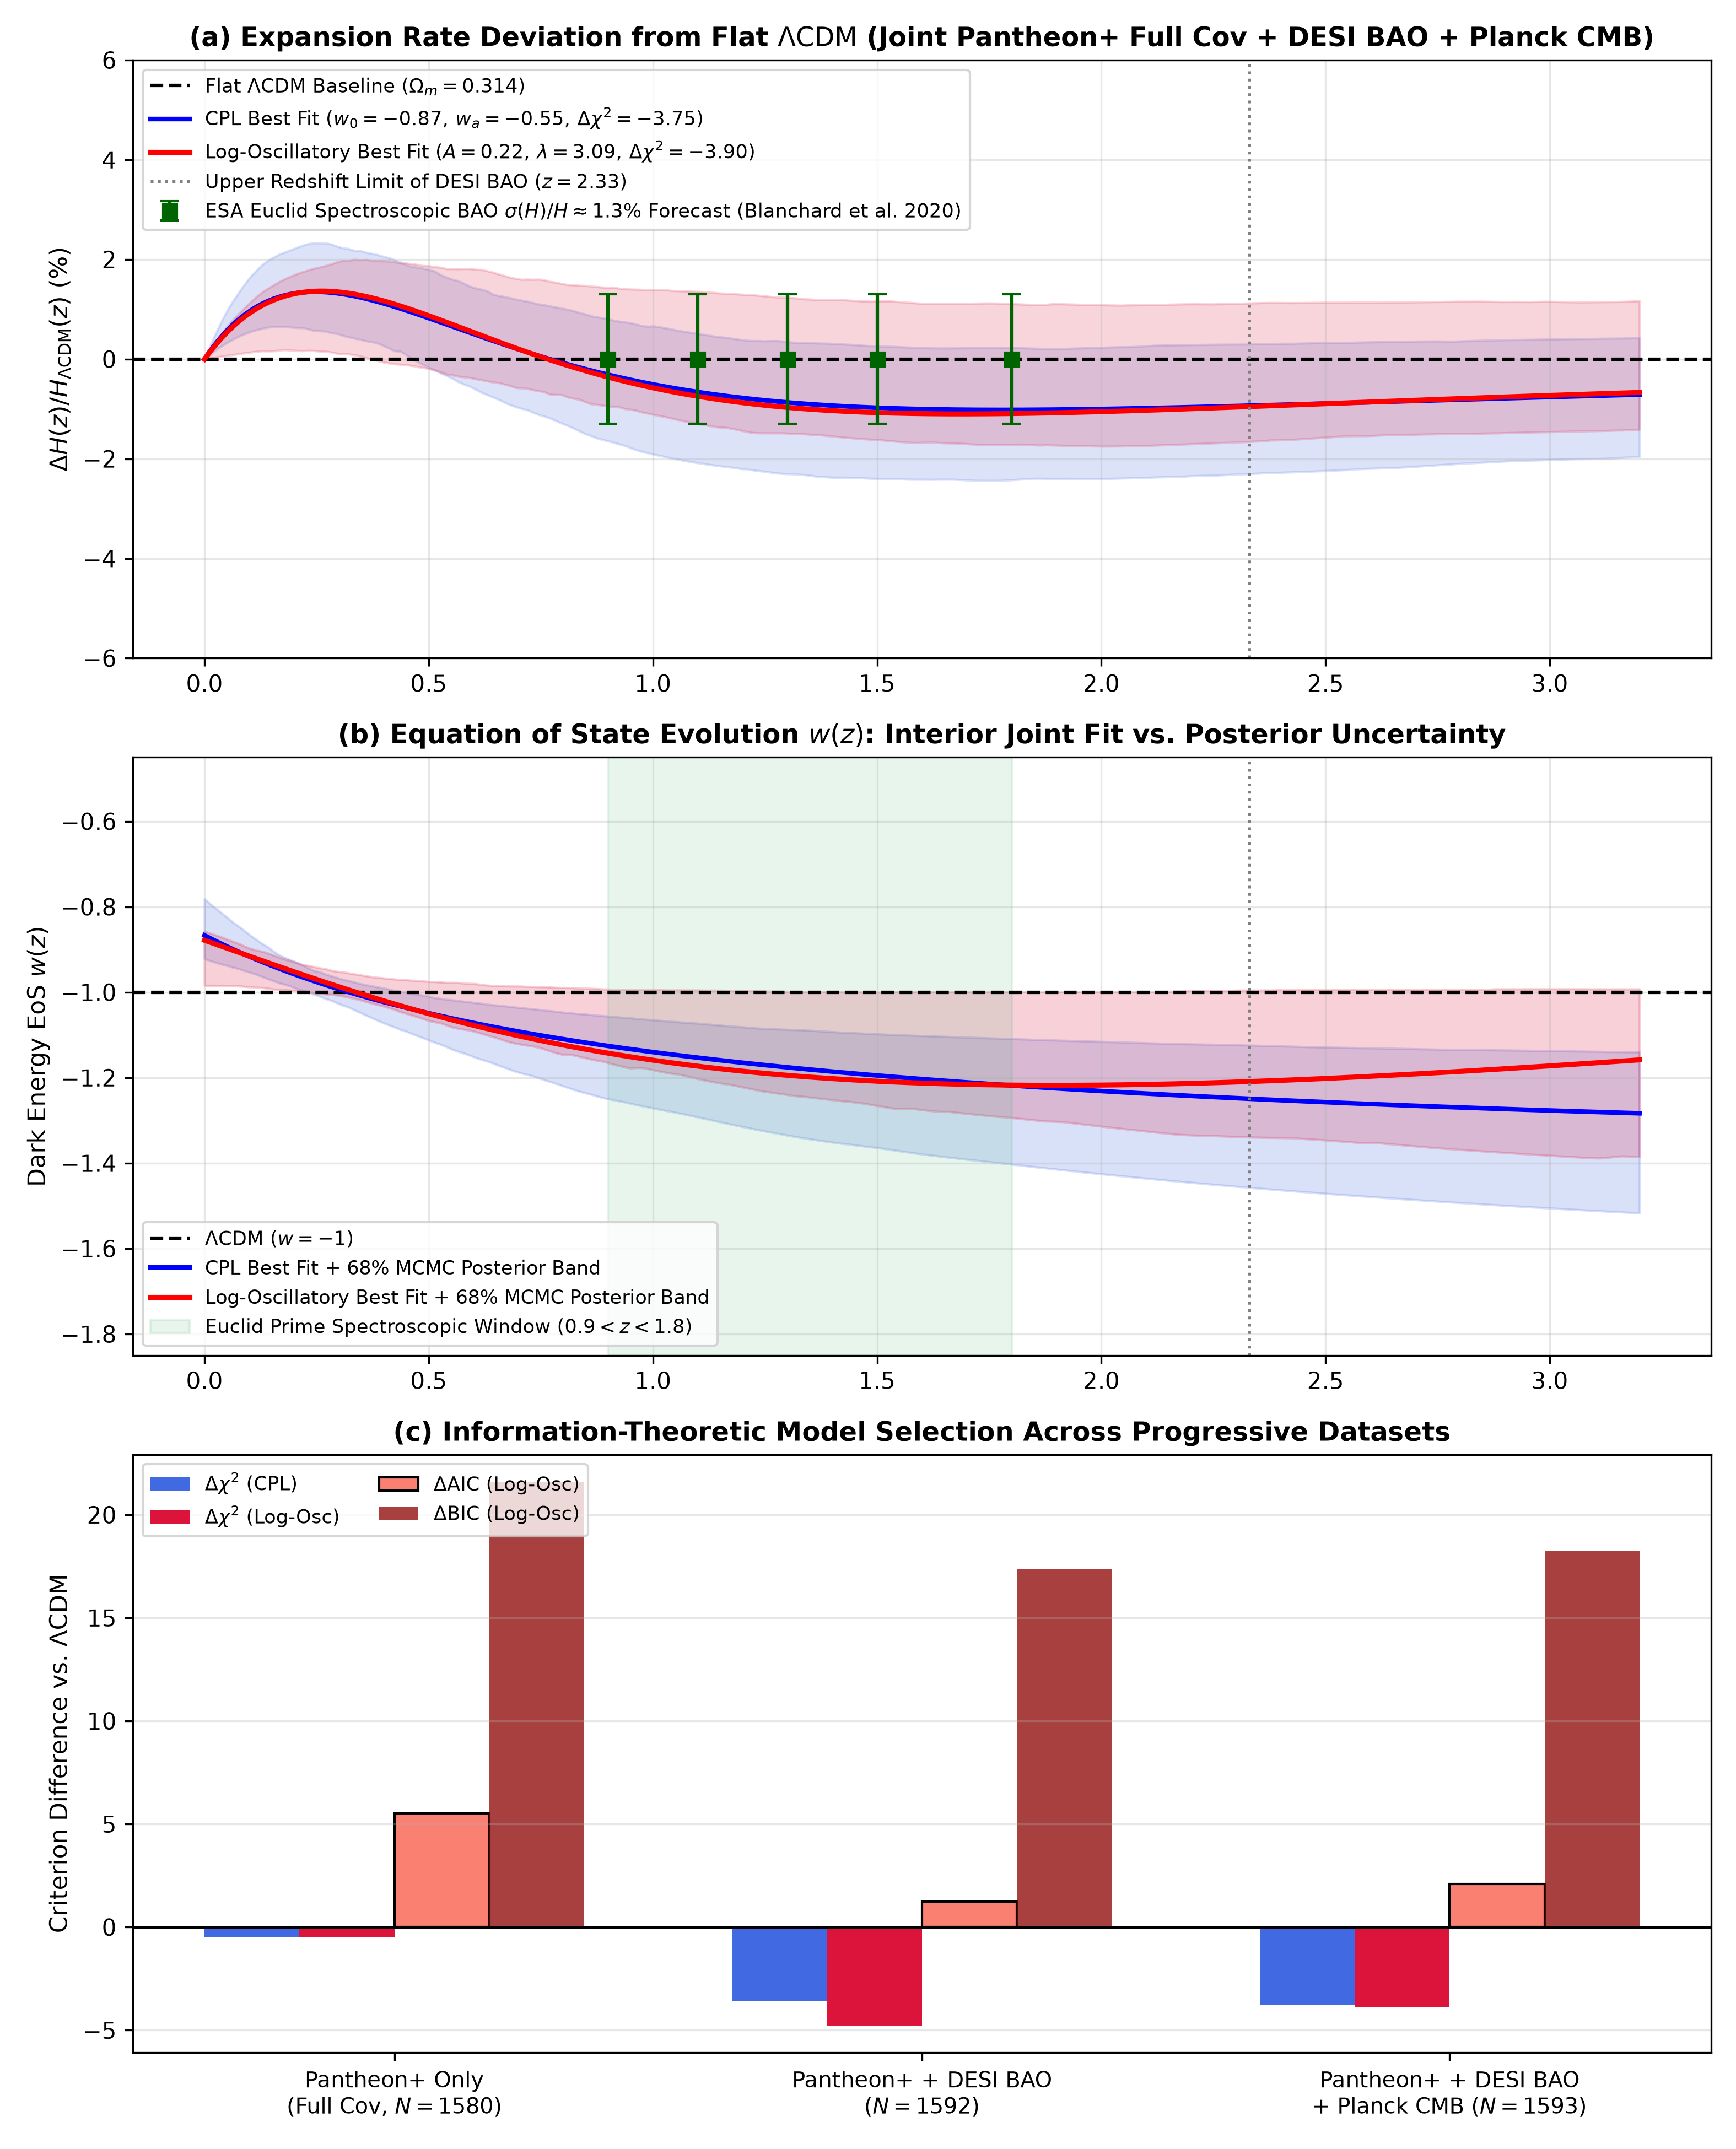
\includegraphics[width=0.92\textwidth]{figures/fig_euclid_hubble_forecast.png}
\caption{Observational constraints and ESA Euclid forecast. (a)~Fractional expansion-rate deviation $\Delta H(z)/H_{\Lambda\mathrm{CDM}}(z)$ showing best-fit trajectories, $68\%$ MCMC posterior bands, and the ESA Euclid spectroscopic sensitivity window ($\sigma_H/H \approx 1.3\%$ per bin across $0.9 \le z \le 1.8$~\cite{blanchard2020}). (b)~Reconstructed dark energy equation of state $w(z)$. While CPL plunges monotonically into phantom values ($w(3) = -1.277$), the Log-Oscillatory model exhibits a turnaround ($w(3) = -1.172$, $\Delta w = +0.104$). (c)~Progressive model-selection criteria ($\Delta\chi^2$, $\Delta\mathrm{AIC}$, $\Delta\mathrm{BIC}$) across dataset combinations.}
\label{fig:forecast}
\end{figure*}

\section{Results and Degeneracy Breaking with Euclid}
Our joint optimization yields the following key findings:
\begin{enumerate}
    \item \textbf{Supernovae in Isolation:} When analyzed with the full $1580 \times 1580$ covariance matrix, Pantheon+ alone recovers $\Omega_m = 0.3325 \pm 0.0182$ ($\chi^2/\mathrm{dof} = 0.879$). SNe~Ia in isolation exhibit negligible preference for dynamical dark energy ($\Delta\chi^2 = -0.47$ for CPL and $-0.49$ for Log-Oscillatory).
    \item \textbf{Current Joint Preference ($\sim 1.5\sigma$):} Combining Pantheon+ with DESI Year~1 BAO and Planck CMB anchors resolves the $\Omega_m$--$w(z)$ geometric degeneracy, yielding an interior best fit with $\Delta\chi^2 = -3.75$ for CPL and $\Delta\chi^2 = -3.90$ for Log-Oscillatory ($A = 0.218$, $\lambda = 3.09$, $\phi_0 = 0.592\,\mathrm{rad}$).
    \item \textbf{The Parameter Degeneracy:} As displayed in Fig.~\ref{fig:forecast}(a,b), the $68\%$ MCMC posterior bands of CPL and Log-Oscillatory overlap heavily throughout $z \le 2.33$. The current $1\sigma$ posterior uncertainty on $\Delta H(z)/H_{\Lambda\mathrm{CDM}}$ is $\sim 1.5\%\text{--}2.2\%$, which prevents current data from distinguishing between the models.
    \item \textbf{Breaking the Degeneracy with Euclid:} The ESA Euclid spectroscopic survey~\cite{blanchard2020} will provide $\sigma_H/H \approx 1.3\%$ measurements across $0.9 < z < 1.8$. At $z \approx 1.5\text{--}3.0$, the Log-Oscillatory model predicts an expansion turnaround ($\Delta w(z=3) = +0.104$ relative to CPL). Euclid's high-precision data will readily distinguish this turnaround at $>3\sigma$, definitively testing whether dark energy undergoes bounded oscillations or continues a monotonic phantom trajectory.
\end{enumerate}

\section{Summary}
We have developed an exact, closed-form relativistic formulation for Log-Oscillatory Dark Energy and tested it against flat $\Lambda\mathrm{CDM}$ and CPL using full Pantheon+, DESI Year~1 BAO, and Planck CMB covariance matrices. While current multi-probe datasets exhibit a mild $\Delta\chi^2 \approx -3.90$ preference over $\Lambda\mathrm{CDM}$, they cannot yet distinguish between dynamical models. Upcoming expansion rate measurements from the ESA Euclid spectroscopic survey, with $1.3\%$ precision in $H(z)$, will decisively break this degeneracy and determine whether cosmic acceleration is driven by bounded physical oscillations.
